\documentclass[11pt,a4paper,onecolumn,final]{article}

%OT1 is the default font encoding of memoir class
%It is generally advised to put it before inputenc
%\usepackage{kerkis}
\usepackage[T1]{fontenc}

%Input encoding for typing directly Greek characters
%Other values for the option: latin1, ascii, ansinew
%It is generally advised to put it before babel
\usepackage[utf8]{inputenc}

%MAIN Language the LAST one
\usepackage[greek,english]{babel}

%\usepackage{kerkis}

%The teubner package extends the facilities offered by the CB Greek fonts
%NOTE: This includes also the graphicx package!
%NOTE: When the teubner package is loaded, command \cap (denoting set intersection) is overwritten
%NOTE: TEUBNER.STY FILE HAS BEEN CHANGED A BIT IN LINES 255-257 WITH 3 REPLACEMENTS \cap -> \capt
\usepackage{teubner}

%Package for displaying math
\usepackage{amsmath}

%Loading a superset of amsfonts
\usepackage{amssymb}

%Provides an enhanced version of \newtheorem
%1.Defines * for unnumbered environments
%2.Defines a proof environment
%3.Defines plain, definition, and remark theorem styles
\usepackage{amsthm}

%Allows text in eps files to be replaced with LATEX symbols
\usepackage{psfrag}

%An extension of the cite package, compatible with the IEEEtranN bibliography style
\usepackage[numbers,sort&compress]{natbib}

\makeatletter\let\c@lofdepth\relax\let\c@lotdepth\relax\makeatother
\usepackage[small,bf,tight]{subfigure}

%Math symbols of the dsfont style. Enables the use of \mathds{}
\usepackage{dsfont}

%Defines several symbols in text mode (e.g. the \textreferencemark for use in the itemize environment)
\usepackage{textcomp}

%Enables the Ralph Smith's Formal Script font in math mode via the \mathscr{} command
\usepackage{mathrsfs}

\usepackage{geometry}
%PDF VIEW
\geometry{total={210mm,297mm},left=25mm,right=25mm,bindingoffset=0mm, top=25mm,bottom=25mm}
%PRINT
%\geometry{total={210mm,297mm},left=20mm,right=20mm,bindingoffset=10mm, top=25mm,bottom=25mm}

\usepackage[breaklinks=true,colorlinks=true,
%linkcolor=blue,urlcolor=blue,citecolor=blue,% PDF VIEW
linkcolor=black,urlcolor=black,citecolor=black,% PRINT
bookmarks=false,bookmarksopenlevel=2]{hyperref}

%Convenient language switch
\newcommand{\gr}[1]{\foreignlanguage{greek}{#1}}
\newcommand{\en}[1]{\foreignlanguage{english}{#1}}

%\newtheorem{definition}{Ορισμός}
\newtheorem{definition}{Definition}
\newtheorem{example}{Example}
\newtheorem{exercise}{Exercise}
%\newtheorem{lemma}{Λήμμα}
\newtheorem{lemma}{Lemma}
%\newtheorem{proof}{Proof}
\newtheorem{notation}{Notation}
\newtheorem{problem}{Problem}
%\newtheorem{proposition}{Πρόταση}
\newtheorem{proposition}{Proposition}
\newtheorem{remark}{Remark}
\newtheorem{solution}{Solution}
\newtheorem{summary}{Summary}
\newcommand{\argmax}{\arg\!\max}
%\addto\captionsgreek{\renewcommand{\chaptername}{Κεφάλαιο}}
%\addto\captionsgreek{\renewcommand{\tablename}{Πίνακας }}
%\addto\captionsgreek{\renewcommand{\proofname}{Απόδειξη }}

\makeatletter
%\renewcommand{\fnum@figure}{Σχήμα \thefigure}
%\renewcommand{\fnum@table}{Πίνακας \thetable}
\makeatother
\begin{document}

%COVER PAGE%%%%%%%%%%%%%%%%%%%%%%%%%%%%%%%%%%%%%%%%%%%%%%%%%%%%%%%%%%%%%%%%%%%%%
\thispagestyle{empty}
{\sffamily\centering\Large

\vspace{\fill}

{\Large Aristotle University of Thessaloniki\\
Department of Electrical and Computer Engineering\\
Telecommunications Division}\\[0.5cm]


\vspace{2.0cm}

{\LARGE Andreas Odontopoulos}\\[0.3em]
{\normalsize AEM: \texttt{<fill in your AEM>}}

\vspace{3.5cm}


{\LARGE Communication Systems II}\\[1em]

{\large Seeing Signals: An Interactive RF Constellation Visualiser\\[0.2em]
and a Synthetic Image Dataset for Automatic Modulation Classification}

\vspace{3.5cm}

%\vspace{\fill}

%
}
%%COVER PAGE%%%%%%%%%%%%%%%%%%%%%%%%%%%%%%%%%%%%%%%%%%%%%%%%%%%%%%%%%%%%%%%%%%%%%

\newpage


%ABSTRACT%%%%%%%%%%%%%%%%%%%%%%%%%%%%%%%%%%%%%%%%%%%%%%%%%%%%%%%%%%%%%%%%%%%%%%%
\begin{center}{\large\bfseries Abstract}\end{center}
\noindent We present an end-to-end pipeline for Automatic Modulation Classification (AMC)
built around a custom interactive ground-station visualiser. A Qt/C++ application uses the
\texttt{liquid-dsp} library to synthesise sixteen digital modulation schemes at complex
baseband, corrupts each symbol with a configurable chain of physical impairments (additive
white Gaussian noise, oscillator phase noise, I/Q imbalance and a coherent continuous-wave
interferer), and renders the resulting constellation as a phosphor-style image. Driven in
an automated mode, the same engine exports a labelled dataset of $3072$ images
($224\times224$) spanning a five-dimensional sweep of modulation and impairment severity.
We analyse each impairment model mathematically, validate the additive-noise channel
against the theoretical symbol-error probability of square QAM, and train two image
classifiers --- a ResNet-18 convolutional network and a LoRA fine-tuned SmolVLM-256M
vision-language model --- reaching $80\%$ and $55\%$ validation accuracy respectively. The
confusion structure exposed a modelling error in our hexagonal-QAM constellations, which we
trace and correct. All artefacts are reproducible from the accompanying application.
%ABSTRACT%%%%%%%%%%%%%%%%%%%%%%%%%%%%%%%%%%%%%%%%%%%%%%%%%%%%%%%%%%%%%%%%%%%%%%%

\newpage

%\tableofcontents


\section{Introduction and project overview}

\subsection{Aim}
Automatic Modulation Classification (AMC) is the task of identifying the modulation scheme
of a received radio signal without prior agreement between transmitter and receiver. It is a
building block of cognitive radio, spectrum monitoring and electronic warfare, and is
increasingly tackled with deep learning applied either to raw I/Q sequences or to image
representations of the signal \cite{OShea2018}. The aim of this project is to build, from
the ground up, the entire chain required to attack AMC as an image-classification problem:
a signal generator, a physically-motivated channel model, a rendering/export stage, and
finally the learned classifiers.

\subsection{How it was achieved}
Rather than downloading a ready-made dataset, we implemented an interactive ground-station
visualiser as a native Qt~6 / C++ application. The digital-signal-processing core is built
on the open-source \texttt{liquid-dsp} library \cite{liquiddsp}, which provides the
modulator/demodulator (\emph{modem}) objects used throughout. The application runs two
pipelines that share the same engine: a \emph{live} mode, in which the user explores the
effect of each impairment on the constellation in real time, and an automated \emph{dataset}
mode, in which the engine sweeps every modulation/impairment combination and exports a
labelled image for each. The full pipeline is therefore self-contained:
\begin{center}
bits $\rightarrow$ I/Q symbols $\rightarrow$ impaired constellation $\rightarrow$ labelled
image $\rightarrow$ classifier.
\end{center}

\subsection{On the choice of models}
We make no claim that the two classifiers chosen are optimal; they were selected
pragmatically to contrast two paradigms on identical data. The first is a compact,
conventional convolutional network (ResNet-18 \cite{He2016}), the natural baseline for
$224\times224$ images. The second is a small instruction-tuned vision-language model
(SmolVLM-256M \cite{SmolVLM2025}), fine-tuned with Low-Rank Adaptation (LoRA) \cite{Hu2021},
to probe whether a general multimodal model can ``read'' a constellation. Both are small
enough to train on modest hardware; a systematic architecture search was out of scope.

\section{The signal and data-generation pipeline}
\label{sec:pipeline}
This section follows a single symbol through the engine, from bits to a rendered point, and
then describes how the labelled dataset is assembled.

\subsection{From bits to I/Q symbols}
At complex baseband a digitally-modulated signal is a sequence of complex symbols
$s = I + jQ$, where the in-phase $I$ and quadrature $Q$ components modulate two orthogonal
carriers. Each modem maps $\log_2 M$ input bits to one of $M$ constellation points. We
expose the sixteen schemes required by the assignment: amplitude-shift keying (4/8-ASK),
phase-shift keying (BPSK, QPSK), square and cross quadrature-amplitude modulation
(16/32/64/128/256-QAM), amplitude/phase-shift keying (16/32/64/128-APSK) and hexagonal QAM
(4/16/64-HQAM). All built-in modems are normalised to unit average symbol energy,
$E[|s|^2]=E_s=1$, so that the signal-to-noise ratio is well defined and identical across
schemes. Figure~\ref{fig:atlas} shows one clean example of each scheme, captured directly
from the application.

\begin{figure}[htbp]
\centering
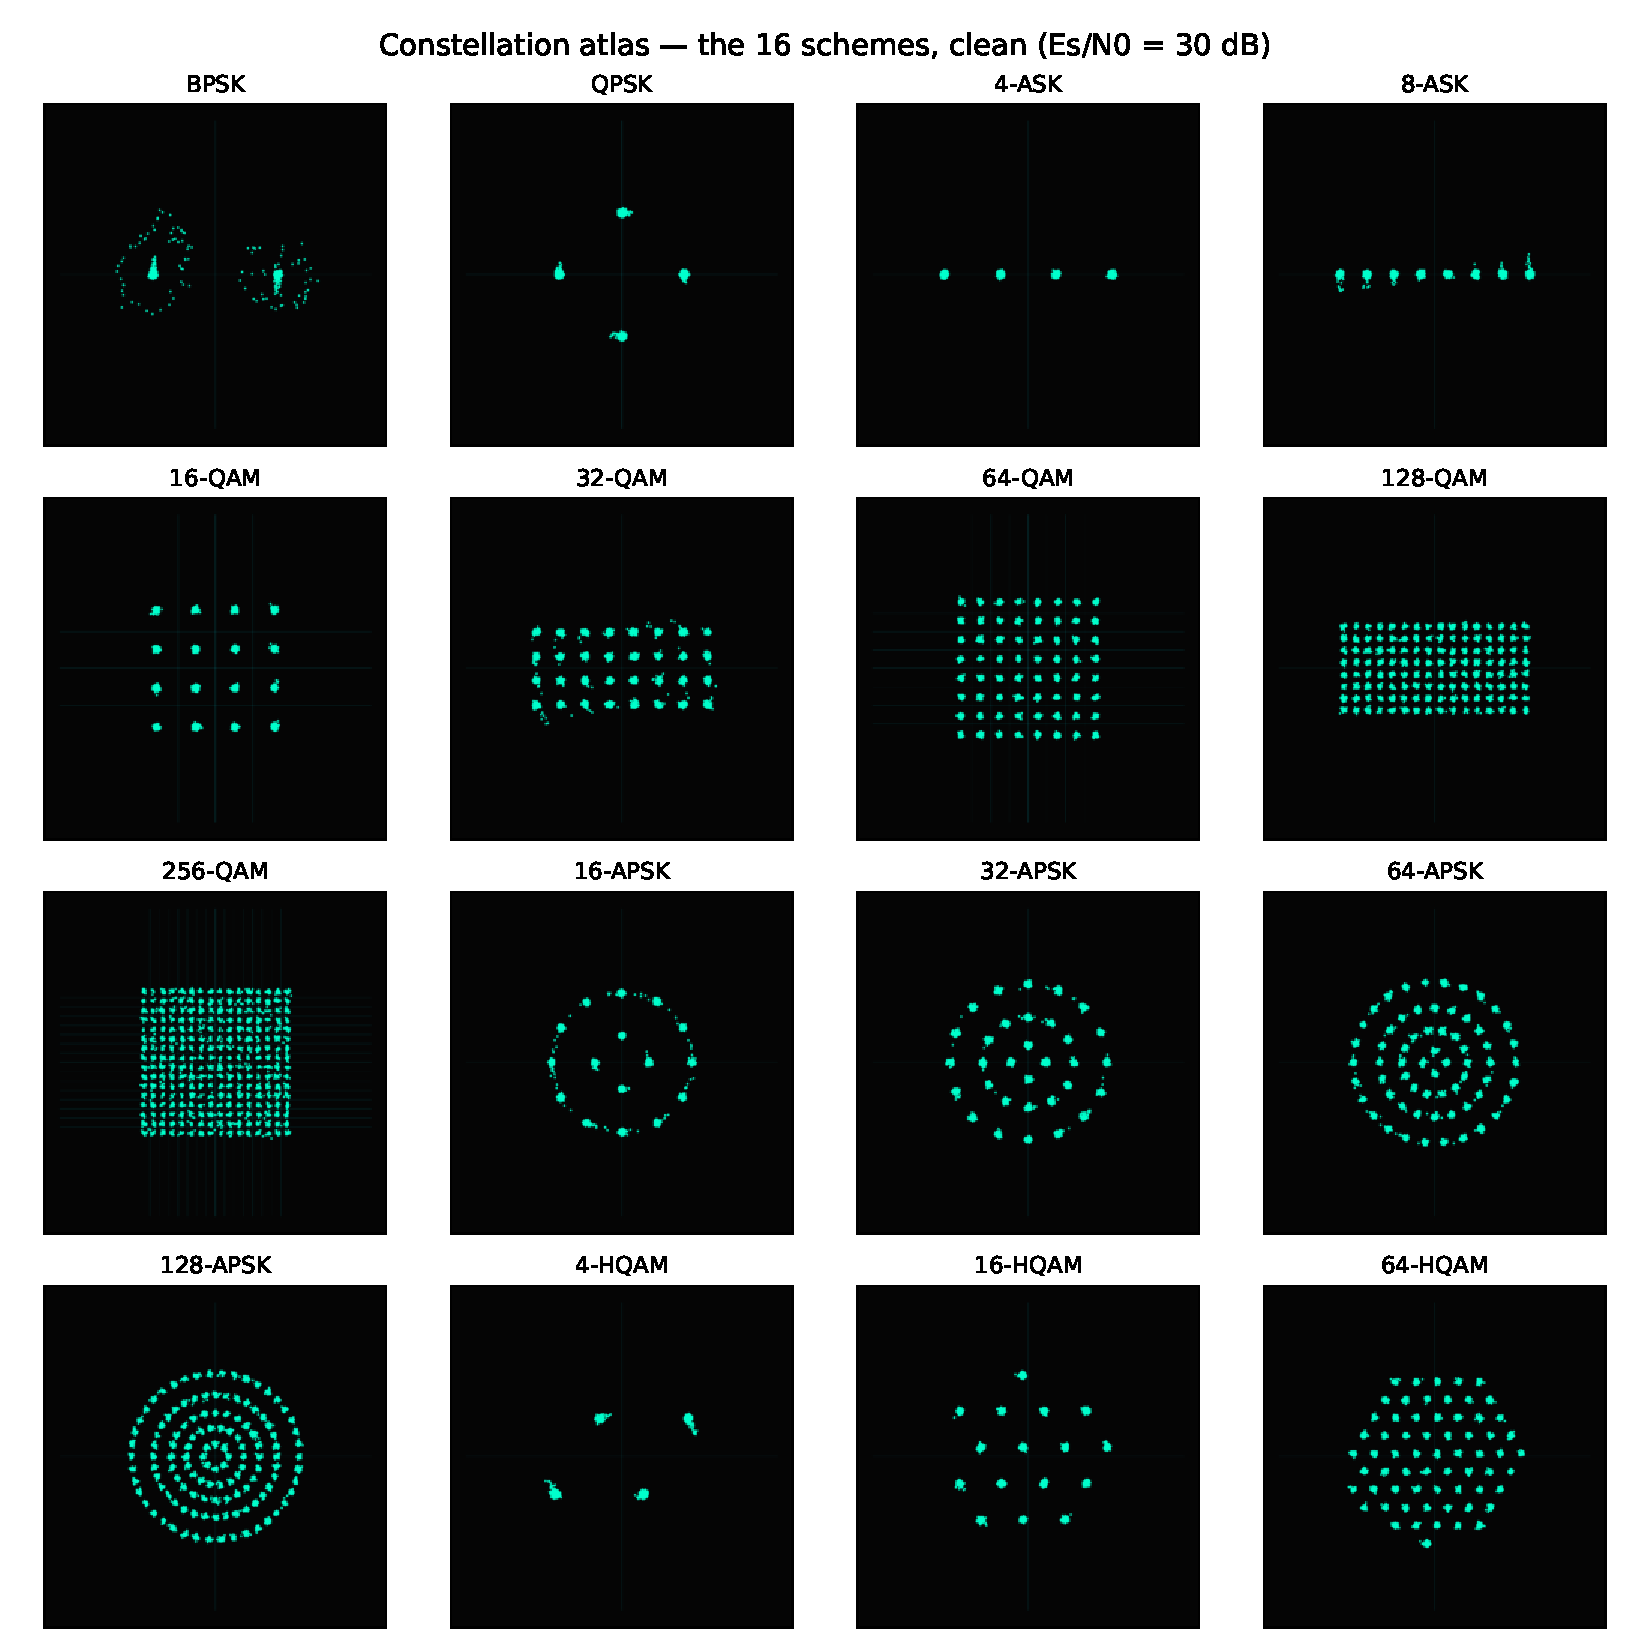
\includegraphics[width=0.92\columnwidth]{figures/constellation_atlas.pdf}
\caption{The sixteen modulation schemes rendered by the application at $E_s/N_0=30$~dB with
no other impairments. The amplitude (ASK), phase (PSK), square (QAM), circular (APSK) and
hexagonal (HQAM) geometries are clearly distinct.}
\label{fig:atlas}
\end{figure}

\subsection{The channel: a chain of physical impairments}
\label{sec:noise}
The heart of the project is the impairment model. A transmitted symbol is passed through
four cascaded effects, applied in the physical order in which they occur along the link:
transmitter I/Q imbalance, channel phase rotation, external interference and, finally,
receiver thermal noise. Let the ideal symbol be $(I,Q)$.

\paragraph{(1) I/Q imbalance.} Gain and phase mismatch between the in-phase and quadrature
branches of the front end is modelled, with the in-phase branch as reference, by
\begin{equation}
\hat I = I, \qquad \hat Q = g\,(Q\cos\varphi - I\sin\varphi),
\end{equation}
where $g$ is the relative gain and $\varphi$ the orthogonality error. This shears and scales
the constellation (Figure~\ref{fig:noise}, third row).

\paragraph{(2) Phase noise.} A free-running oscillator does not have a perfectly stable
phase; its phase performs a random walk (a Wiener process),
$\theta[n]=\theta[n-1]+w[n]$ with $w\sim\mathcal{N}(0,\sigma_\Delta^2)$, whose variance grows
without bound. In practice a carrier-recovery loop tracks and removes the slow drift, leaving
a \emph{bounded residual}. We model this residual as a first-order autoregressive
(Ornstein--Uhlenbeck) process,
\begin{equation}
\theta[n] = (1-\alpha)\,\theta[n-1] + \sigma_{\text{step}}\,w[n],\qquad w\sim\mathcal{N}(0,1),
\end{equation}
whose stationary variance is $\operatorname{Var}(\theta)=\sigma_{\text{step}}^2/(\alpha(2-\alpha))$.
We therefore set $\sigma_{\text{step}}=\sigma_\theta\sqrt{\alpha(2-\alpha)}$ so that
$\sigma_\theta$ is the target residual RMS phase; $\alpha$ (here $0.02$) sets the loop memory
($\sim 1/\alpha$ symbols). The symbol is rotated by $\theta[n]$. Unlike an independent
per-symbol jitter, the random walk produces the characteristic rotational smear of
Figure~\ref{fig:noise} (second row) and, crucially, an irreducible error floor
(Section~\ref{sec:sep}).

\paragraph{(3) Continuous-wave interference.} A narrow-band jammer is modelled as a coherent
tone of amplitude $A$ rotating at a fixed normalised offset frequency $f_{\text{off}}$:
$j[n] = A\,e^{\,j 2\pi f_{\text{off}} n}$. Because the tone is coherent, it traces a circle
around each constellation point over time, turning every point into a ring
(Figure~\ref{fig:noise}, fourth row).

\paragraph{(4) Additive white Gaussian noise.} Finally, receiver thermal noise is added as
circularly-symmetric complex Gaussian noise $n=n_I+jn_Q$ with $n_I,n_Q\sim\mathcal{N}(0,\sigma^2)$
i.i.d. The complex noise power is $N_0=E[|n|^2]=2\sigma^2$, hence $E_s/N_0 = 1/(2\sigma^2)$.
To make the user-facing SNR control read $E_s/N_0$ directly we set
\begin{equation}
\sigma = \tfrac{1}{\sqrt2}\,10^{-\text{SNR}/20}
\qquad\Longrightarrow\qquad
\frac{E_s}{N_0}=10^{\,\text{SNR}/10}.
\label{eq:sigma}
\end{equation}
The $1/\sqrt2$ factor matters: omitting it (as an earlier version of the engine did) makes
the link $3$~dB worse than the label, shifting every error-rate curve. Gaussian samples are
drawn with the Box--Muller transform. The rows of Figure~\ref{fig:noise} isolate each
impairment on a 16-QAM constellation.

\begin{figure}[htbp]
\centering
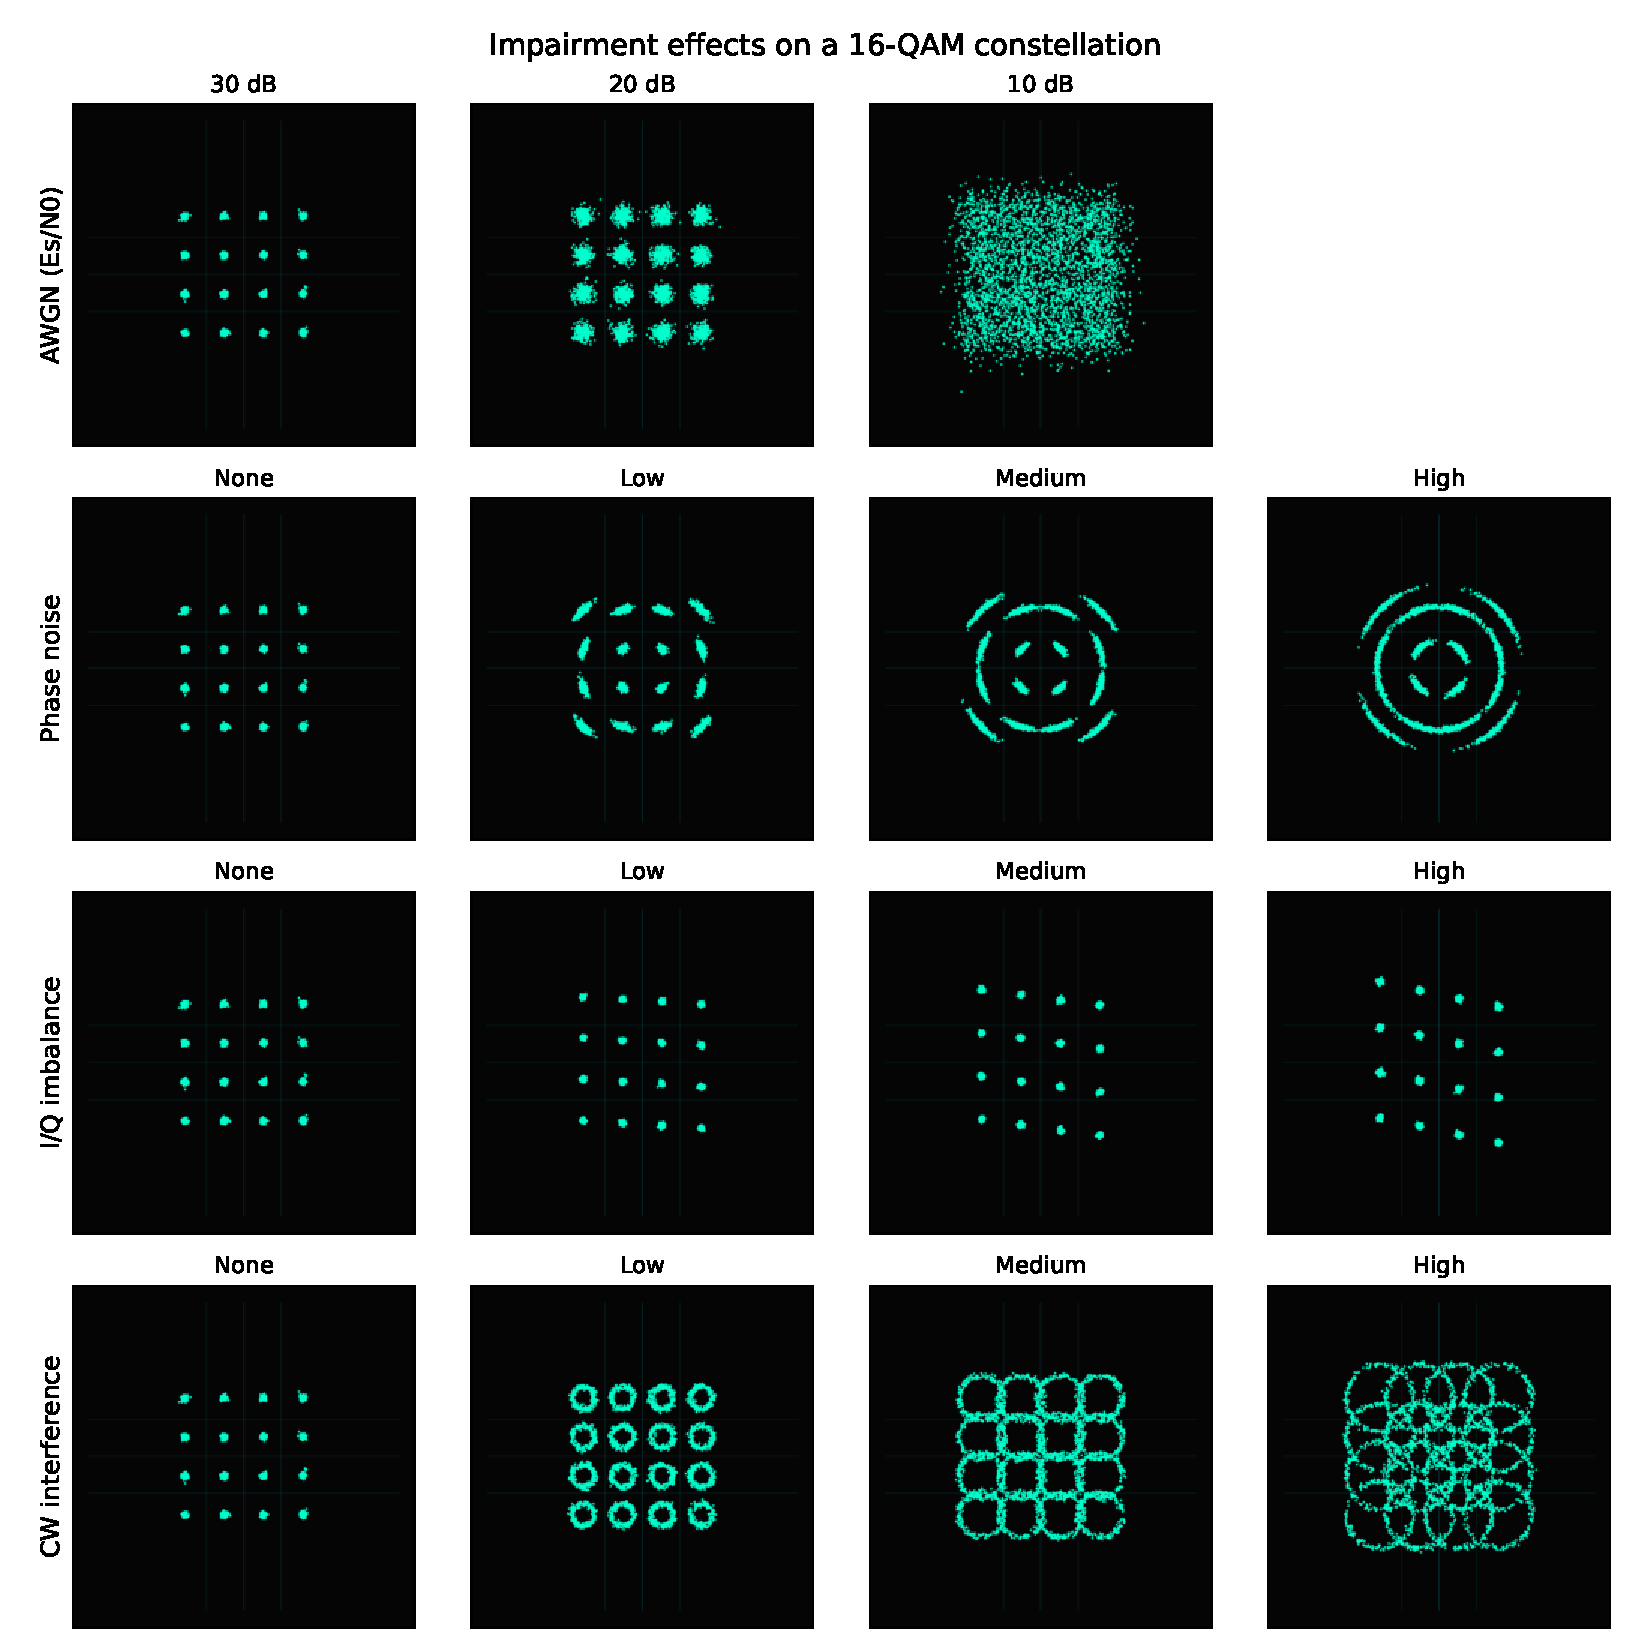
\includegraphics[width=0.92\columnwidth]{figures/noise_effects.pdf}
\caption{Effect of each impairment on a 16-QAM constellation, captured from the application.
Top to bottom: decreasing $E_s/N_0$ (AWGN cloud); increasing phase noise (rotational smear);
increasing I/Q imbalance (shear); increasing CW interference (each point becomes a ring). The
faint cross/grid lines are the optional decision-boundary overlay
(Section~\ref{sec:dataset}).}
\label{fig:noise}
\end{figure}

\paragraph{Discrete severity levels.} For dataset generation each impairment is quantised to
the four qualitative levels \emph{None/Low/Medium/High}, and the SNR to three levels.
Table~\ref{tab:levels} gives the exact parameter behind each label.

\begin{table}[htbp]
\centering
\caption{Quantitative meaning of the qualitative impairment levels. The SNR uses only the
three non-trivial levels; the three impairments additionally include a ``None'' level.}
\label{tab:levels}
\begin{tabular}{lcccc}
\hline
Severity & $E_s/N_0$ & Phase $\sigma_\theta$ & I/Q $(g,\varphi)$ & Jammer $A$\\
\hline
None   & ---     & $0^\circ$    & $(1.00,\,0^\circ)$    & $0$\\
Low    & $10$~dB & $3.4^\circ$  & $(1.06,\,3.4^\circ)$  & $0.18$\\
Medium & $20$~dB & $6.9^\circ$  & $(1.12,\,6.9^\circ)$  & $0.36$\\
High   & $30$~dB & $10.3^\circ$ & $(1.18,\,10.3^\circ)$ & $0.54$\\
\hline
\end{tabular}
\end{table}

\subsection{Detection: the ``guess''}
For every transmitted symbol the engine also performs hard detection with the
\texttt{liquid-dsp} demodulator, which returns the nearest constellation point by minimum
Euclidean distance. Comparing the transmitted and detected symbols yields the instantaneous
symbol- and bit-error counts that drive the live telemetry and the error-rate measurements
below.

\subsection{Symbol-error probability and the phase-noise floor}
\label{sec:sep}
To validate the channel model we measure the symbol-error probability (SEP) versus
$E_s/N_0$ for the square constellations 16/64/256-QAM, under both no phase noise and high
phase noise, and compare against the textbook expression for square $M$-QAM
\cite{Proakis2008},
\begin{equation}
P_s = 4\Big(1-\tfrac{1}{\sqrt M}\Big)Q\!\left(\!\sqrt{\tfrac{3}{M-1}\tfrac{E_s}{N_0}}\right)
- 4\Big(1-\tfrac{1}{\sqrt M}\Big)^{2} Q^{2}\!\left(\!\sqrt{\tfrac{3}{M-1}\tfrac{E_s}{N_0}}\right),
\end{equation}
with $Q(x)=\tfrac12\operatorname{erfc}(x/\sqrt2)$. Figure~\ref{fig:sep} shows the result.
With the calibrated noise of \eqref{eq:sigma} the simulated AWGN points fall exactly on the
theoretical curves, confirming that the ``SNR'' control is a true $E_s/N_0$. Under high phase
noise the curves no longer fall off indefinitely but flatten into an \emph{error floor}:
beyond a certain SNR the residual phase, not the thermal noise, dominates, and adding power
no longer helps. The floor is highest for 256-QAM and lowest for 16-QAM, since denser
constellations have less angular margin --- a textbook qualitative result reproduced
quantitatively by our engine.

\begin{figure}[htbp]
\centering
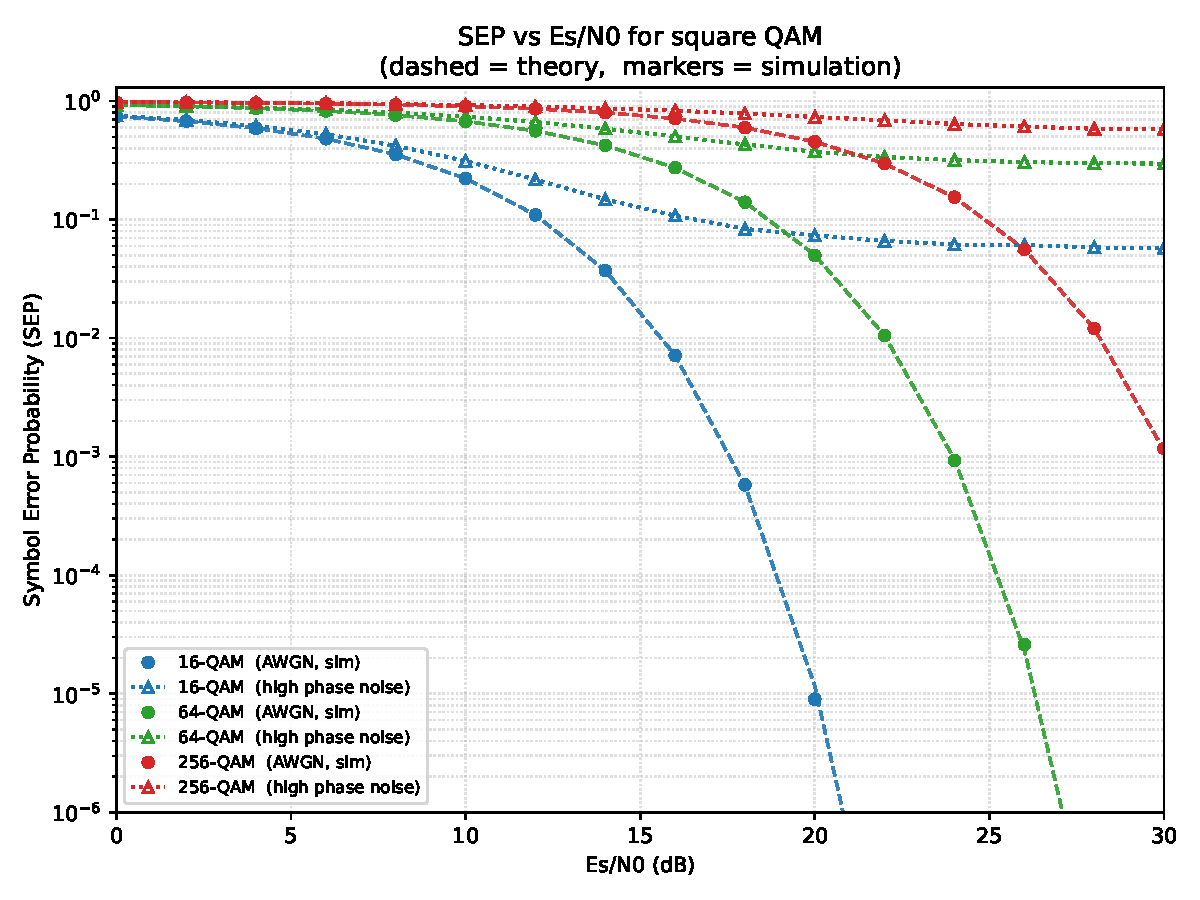
\includegraphics[width=0.85\columnwidth]{figures/SEP_vs_SNR.pdf}
\caption{Symbol-error probability versus $E_s/N_0$. Markers are the simulation; dashed lines
are the theoretical square-QAM SEP. The AWGN-only points match theory; the high-phase-noise
curves exhibit an irreducible error floor that worsens with modulation order.}
\label{fig:sep}
\end{figure}

\subsection{A corrected modelling error: hexagonal QAM}
\label{sec:hqam}
An early version of the engine mapped the three hexagonal-QAM schemes (4/16/64-HQAM) onto the
\emph{square} QAM modems of the same order, because \texttt{liquid-dsp} has no built-in
hexagonal constellation. This produced images pixel-identical to ordinary QAM and, as
Section~\ref{sec:amc} shows, the classifier could not separate the two --- which is how we
caught the bug. We corrected it by building true hexagonal constellations on the $A_2$
lattice (basis $e_1=(1,0)$, $e_2=(\tfrac12,\tfrac{\sqrt3}{2})$): we take the $M$
lowest-energy lattice points, centre them, normalise to unit average energy, and load them
into \texttt{liquid-dsp}'s arbitrary-constellation modem. The resulting constellations
(Figure~\ref{fig:hqam}) are now geometrically distinct from square QAM. We verified
numerically that each table is zero-mean, unit-energy, and demodulates losslessly in the
absence of noise.

\begin{figure}[htbp]
\centering
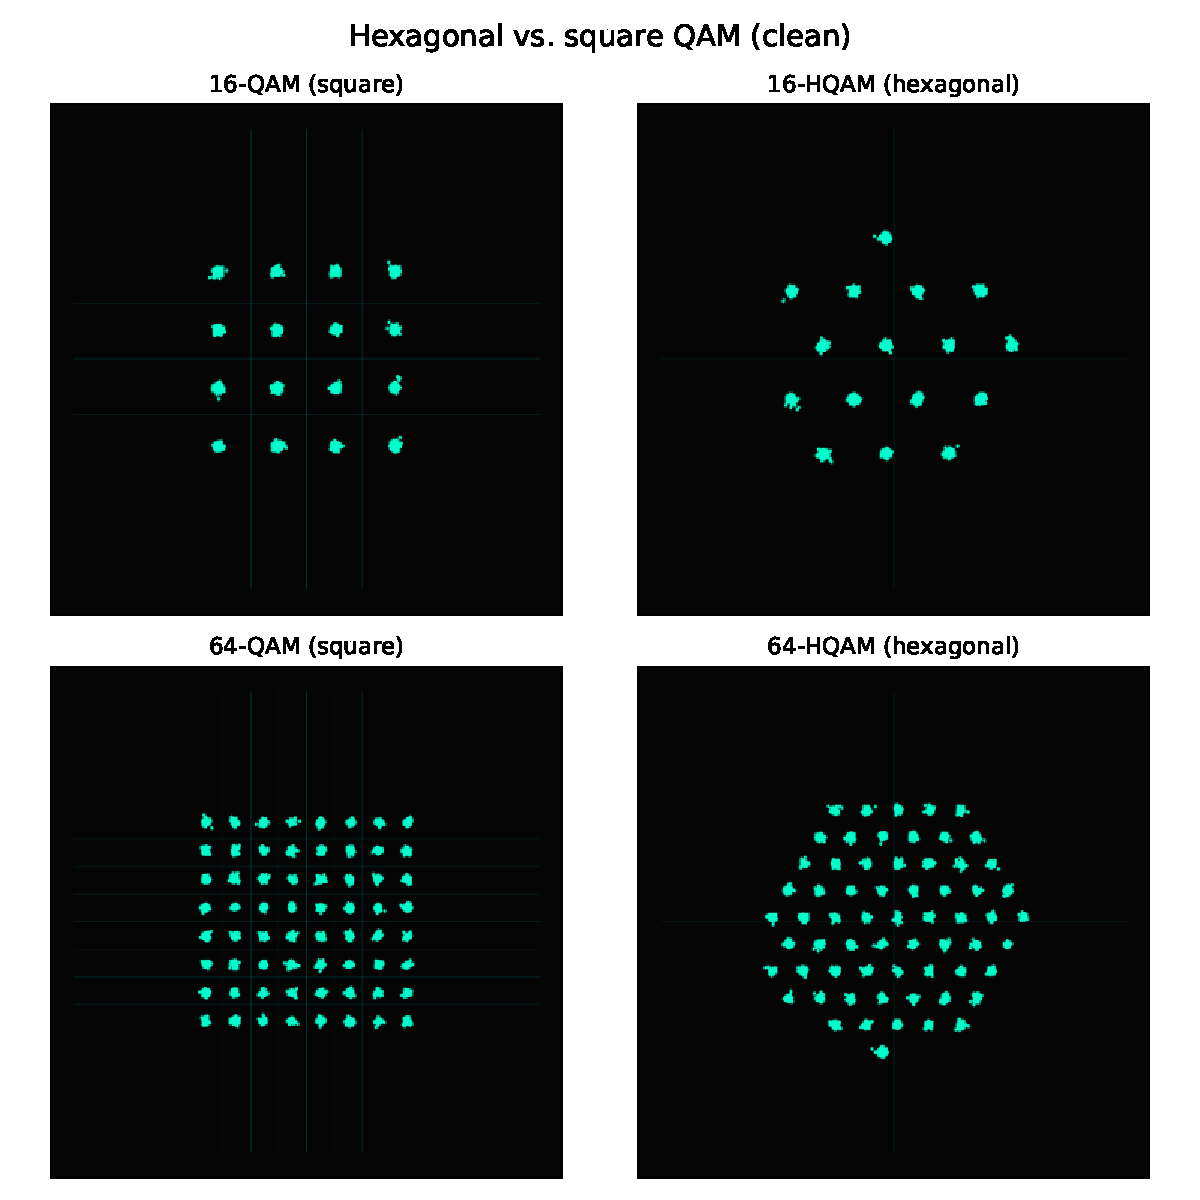
\includegraphics[width=0.7\columnwidth]{figures/hqam_vs_qam.pdf}
\caption{The corrected hexagonal QAM (right column) versus ordinary square QAM (left column).
The hexagonal packing is now visible, removing the aliasing that previously made the two
indistinguishable.}
\label{fig:hqam}
\end{figure}

\subsection{Dataset construction}
\label{sec:dataset}
In dataset mode the engine performs a full five-dimensional sweep: $16$ modulations, $3$ SNR
levels, and $4$ levels each of phase noise, I/Q imbalance and interference, giving
$16\times3\times4\times4\times4=3072$ configurations. For each, the constellation accumulates
a dense cloud of about $3300$ points and is captured as a clean $224\times224$ image (cyan
points on black, no axes or labels --- the native input size of ResNet/VGG-style networks),
together with a CSV row recording the modulation and the four severity labels. A note on
reproducibility: in the run used for the figures here the optional decision-boundary overlay
was left enabled at low opacity, so faint cross/grid lines are visible on the square-QAM
panels; for clean training data this overlay should be disabled (or the application set to
skip it during automation). The export takes a few minutes, the engine having been optimised
to draw a full image roughly four times faster than the initial implementation.

\section{Automatic modulation classification}
\label{sec:amc}

\subsection{Models and training}
Both classifiers are trained on the same $3072$-image dataset with an $80/20$
train/validation split. The convolutional baseline is a ResNet-18 \cite{He2016} trained with
the Adam optimiser and cross-entropy loss for $10$ epochs. The vision-language model is
SmolVLM-256M-Instruct \cite{SmolVLM2025}, adapted to the sixteen-class problem by Low-Rank
Adaptation (LoRA \cite{Hu2021}; rank $16$, $\alpha=32$, dropout $0.05$ on the attention and
MLP projections), trained for $3$ epochs at learning rate $5\times10^{-5}$; only the small
adapter is updated, leaving the $256$M backbone frozen.

\subsection{Convolutional baseline}
The ResNet-18 reaches $80\%$ validation accuracy (macro-F1 $0.78$). Its confusion matrix
(Figure~\ref{fig:cnn}) splits the errors into two clear families:
\begin{itemize}
\item \textbf{Hexagonal vs.\ square QAM aliasing.} 16-HQAM and 64-HQAM have low precision and
bleed into 16-QAM and 64-APSK. This is \emph{not} a weakness of the network: in the dataset
used for training, HQAM was still rendered as square QAM (Section~\ref{sec:hqam}), so the two
classes were literally the same images and could only be guessed at chance. This failure is
precisely what led us to find and fix the constellation bug; with the corrected,
geometrically distinct constellations (Figure~\ref{fig:hqam}) these classes become separable.
\item \textbf{High-order density saturation.} 128-APSK ($13\%$ recall) and 128-QAM ($21\%$
recall) are the densest constellations; 128-QAM is most often confused with 32-QAM. At
$224\times224$ with noise, constellations of $128$--$256$ points blur into near-identical
clouds. This is a genuine information limit of the image representation rather than a
modelling error, and would require higher resolution or per-class SNR control to mitigate.
\end{itemize}
The low-order and structurally distinctive schemes (BPSK, QPSK, 4-HQAM, 16/64/256-QAM) are
classified almost perfectly.

\begin{figure}[htbp]
\centering
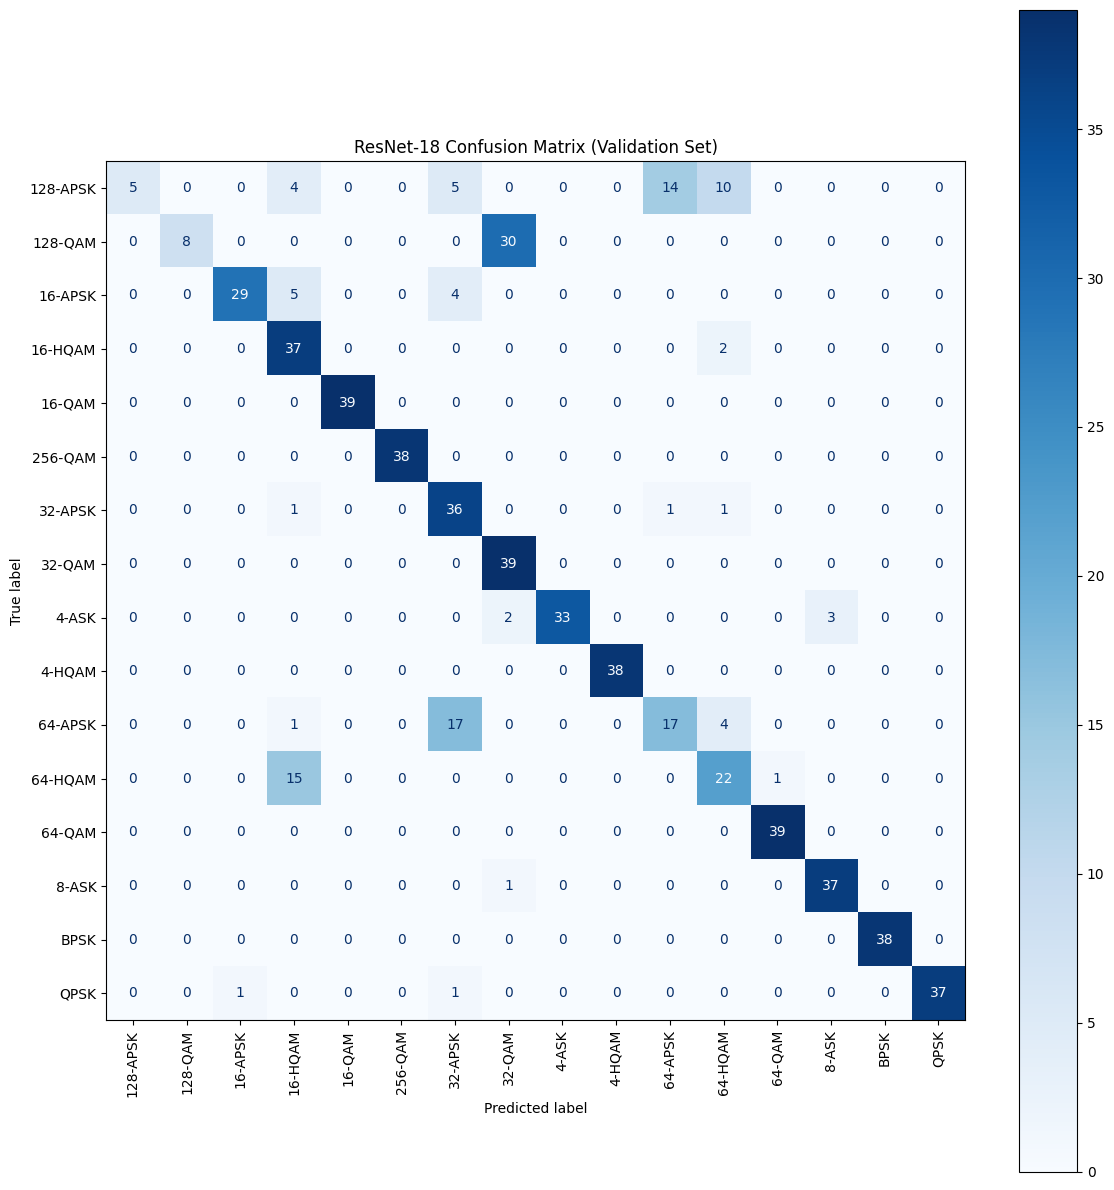
\includegraphics[width=0.8\columnwidth]{figures/cnn_confusion.png}
\caption{ResNet-18 validation confusion matrix. Errors concentrate in (i) the HQAM/QAM
aliasing (since fixed) and (ii) the densest high-order constellations.}
\label{fig:cnn}
\end{figure}

\subsection{Vision-language model}
The LoRA-tuned SmolVLM-256M reaches $55\%$ accuracy (macro-F1 $0.54$). It classifies the
visually distinctive classes well (256-QAM, 64-QAM, 16-QAM and QPSK all above $0.84$ F1) but
struggles far more than the CNN on the APSK family and the high-order schemes
(Figure~\ref{fig:vlm}). This is the expected outcome: a $256$M general-purpose multimodal
model, adapted with a small LoRA on a few thousand images, has neither the inductive bias of
a convolutional network for dense-texture discrimination nor enough task data to acquire it.
The experiment is nonetheless informative --- it shows that a general ``image reader'' can
recover the coarse structure of a constellation but not the fine lattice distinctions that
separate, say, 64-APSK from 64-HQAM.

\begin{figure}[htbp]
\centering
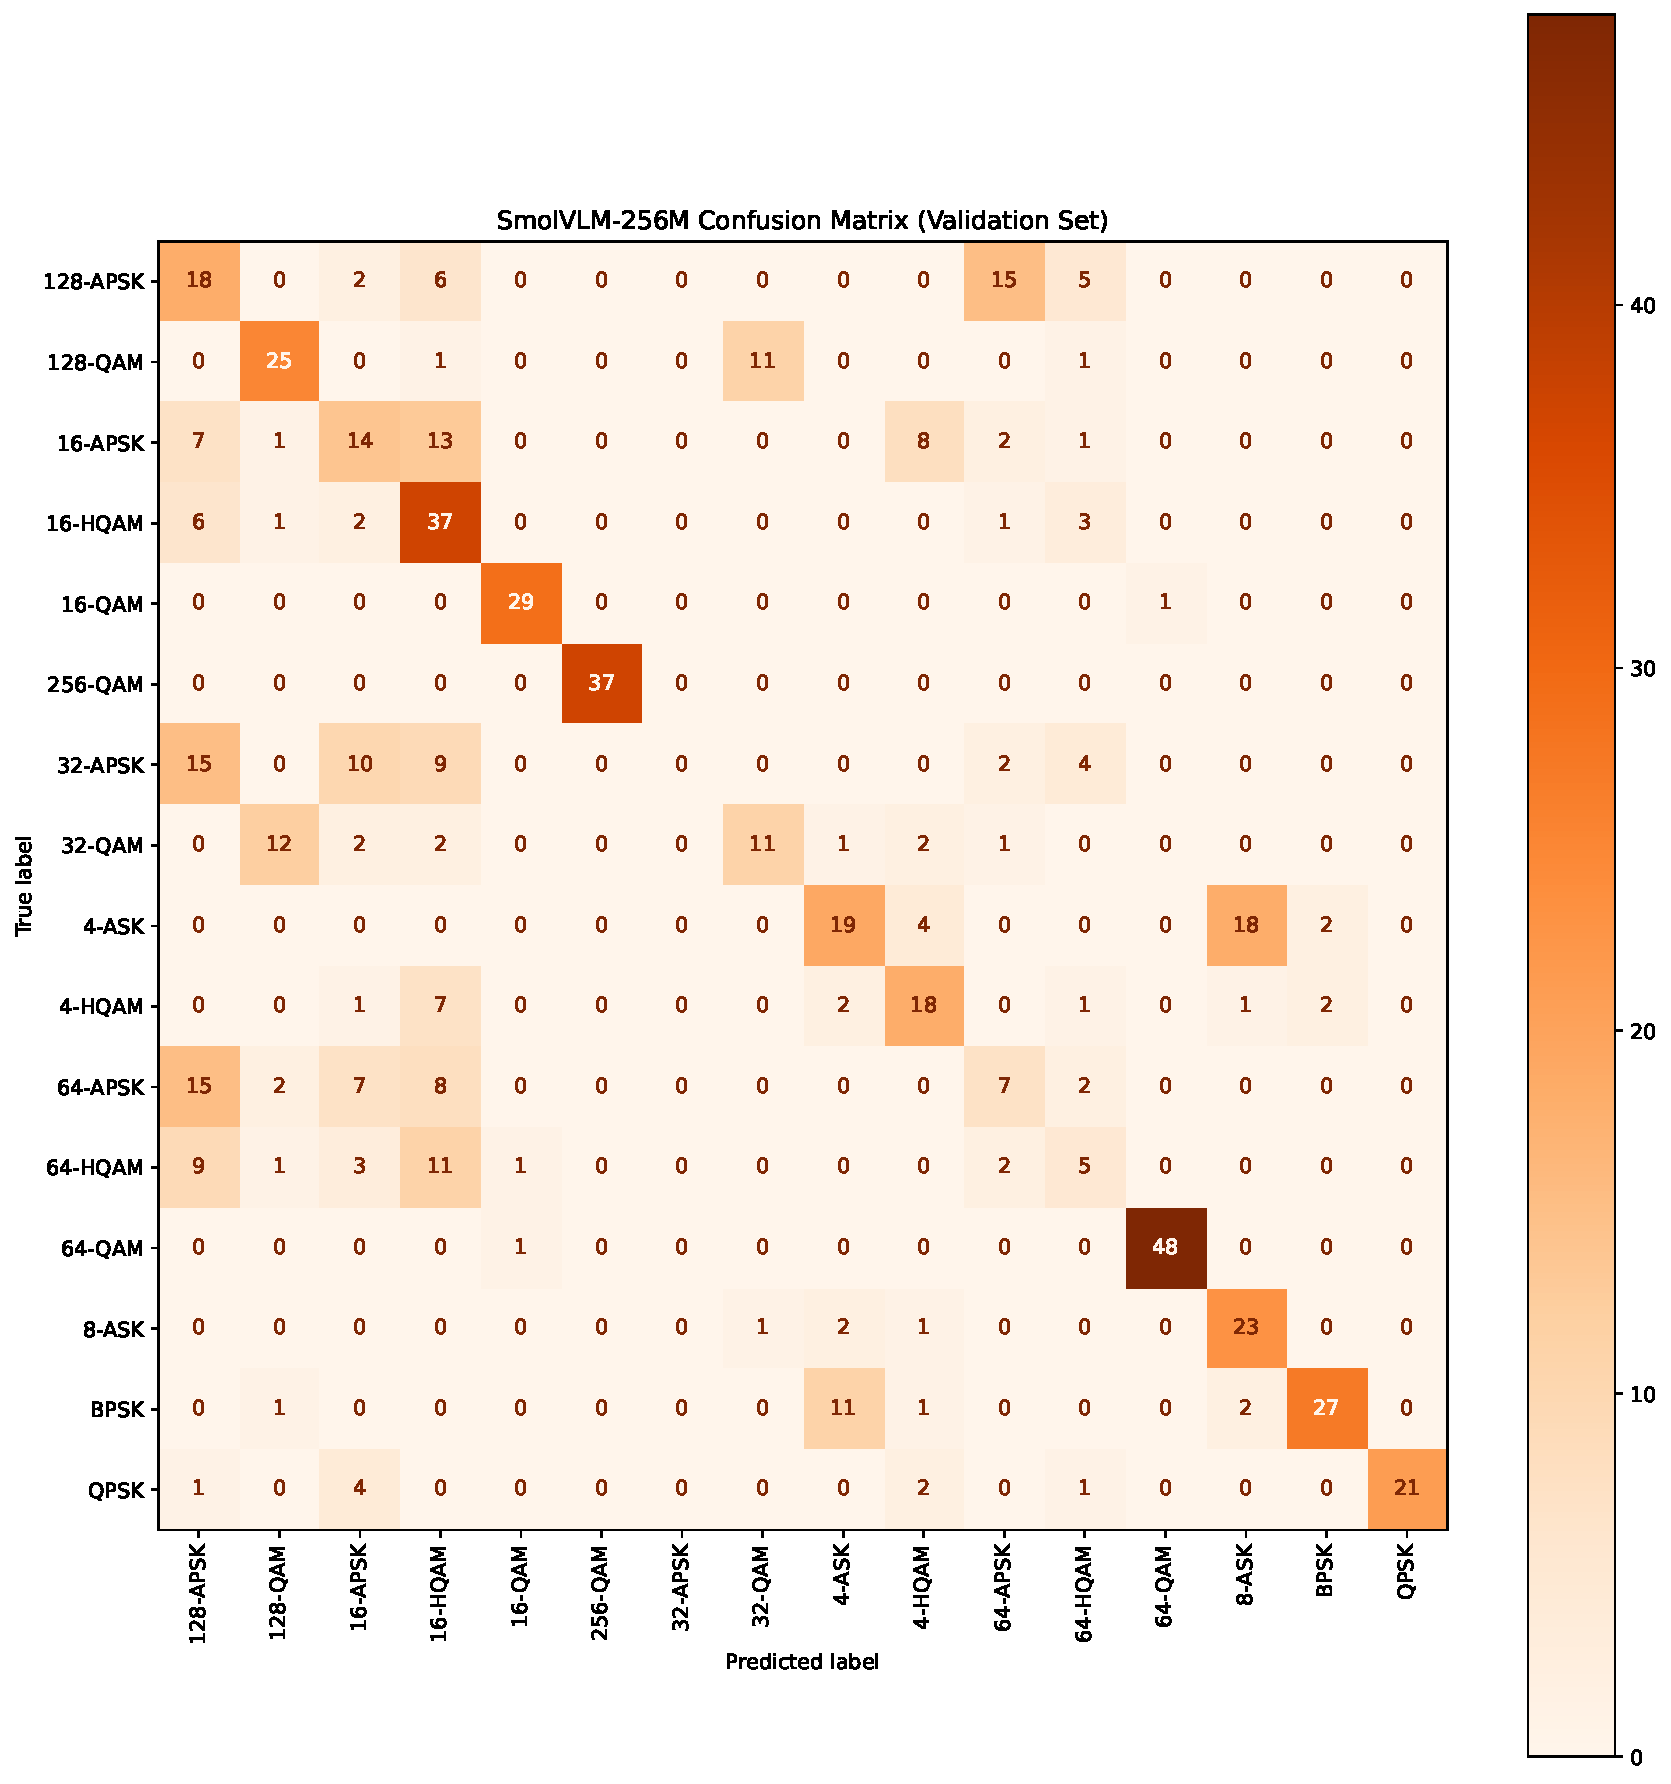
\includegraphics[width=0.8\columnwidth]{figures/vlm_confusion.pdf}
\caption{SmolVLM-256M (LoRA) validation confusion matrix. The model captures coarse
constellation structure but confuses the dense APSK and high-order classes.}
\label{fig:vlm}
\end{figure}

\subsection{Discussion}
On this dataset the convolutional baseline clearly outperforms the fine-tuned VLM ($80\%$
vs.\ $55\%$), which is unsurprising: distinguishing modulations from constellation images is
a fine-grained texture/geometry problem, exactly what convolutional inductive biases are good
at, and the VLM's language head adds little. The most valuable scientific outcome, however,
came from the errors rather than the accuracy: the CNN's inability to separate HQAM from QAM
was a direct, visible symptom of a flaw in our signal generator, which we then corrected at
the source.

\section{The application}
The visualiser is a native Qt~6 application with a C++/QML architecture. The DSP engine runs
on a dedicated worker thread so the user interface stays responsive, and exposes its
parameters to the QML front end through Qt's property and signal system. The front end
provides a live constellation page (a phosphor-persistence canvas that imitates an analogue
oscilloscope), a telemetry dashboard (RSSI/SNR/BER/PLR time series), sliders for every
impairment, a serial-port interface for connecting a real radio, and the one-click dataset
and SEP-curve exporters used to produce the data in this report. The application is thus
simultaneously a teaching instrument, a data-generation rig, and the experimental apparatus
behind every figure here.

\section{Conclusion}
We built a complete, self-contained AMC pipeline: a Qt/C++ visualiser that synthesises
sixteen modulations, corrupts them with a mathematically-grounded chain of impairments
(calibrated AWGN, Wiener/Ornstein--Uhlenbeck phase noise, I/Q imbalance and a coherent CW
jammer), and exports a labelled $3072$-image dataset, on which a ResNet-18 and a LoRA-tuned
SmolVLM reach $80\%$ and $55\%$ accuracy. The additive-noise channel was validated against
theory, the phase-noise error floor was reproduced, and a constellation-modelling error
revealed by the classifier was traced and corrected. Natural extensions include retraining on
the corrected hexagonal constellations, adding multipath fading and carrier-frequency offset
to the channel, and raising the image resolution to relieve the high-order density
saturation.





%\renewcommand\bibname{\gr{Βιβλιογραφία}}
\bibliographystyle{IEEEtranN}
\en{\bibliography{sample}}

\end{document}